\documentclass[12pt,a4paper,oneside]{article}

\usepackage{graphicx}
\usepackage{hyperref}
\usepackage{multicol}
\usepackage[portuguese]{babel}
\usepackage{float}

\begin{document}

\begin{center}


\includegraphics[width=0.7\textwidth]{Ita-logo.png}

{\Large \bf INSTITUTO TECNOLÓGICO DE AERONÁUTICA}

{\Large DEPARTAMENTO DE TEORIA DA COMPUTAÇÃO (IEC-T)}\\
{LABORATÓRIO 3 - ORDENAÇÃO}\\[2.0cm]

\vspace{1cm}

{\bf \large Comparação entre \textit{BubbleSort}, \textit{MergeSort} e \textit{QuickSort}}\\[2.5cm]

{\textbf{T28.4}\\
Leonardo Xavier Dantas (\href{mailto:leonardo.dantas.9092@ga.ita.br}{leonardo.dantas.9092@ga.ita.br})
}\\[2.0cm]

{\bf Professor: Armando Ramos Gouveia}\\[2.5cm]

{\large São José dos Campos - São Paulo}\\[0.2cm]
2024

\end{center}

\newpage

\section{Objetivos}

\quad O objetivo desse relatório é o estudo dos diferentes algorítimos de ordenação, sendo levados em consideração os métodos conhecidos como \textit{MergeSort}, \textit{QuickSort}, \textit{BubbleSort}. Foram analisados o tempo de execução e número de comparações dos algorítimos. 

\section{Procedimentos}

\quad Um gerador de \textit{string} de minha autoria com todas as letras do alfabeto, ambas maiúsculas e minúsculas em foi utilizado para testar os algorítimos.

\quad Os códigos de \textit{QuickSort} e \textit{MergeSort} utilizados foram os fornecidos no Curso de CES-11, ambos de autoria original de Armando Gouveia, adaptados para receberem \textit{array} de \textit{string} e, no caso do MergeSort, foram feitas duas versões, sendo uma delas com o vetor temporário \textit{static}

\quad Foi criado um outro código, permitindo executar repetidamente os algorítimos com diferentes tamanhos de \textit{array}, coletando o tamanho do \textit{array}, o tempo de execução e o número de comparações

\section{Resultados}

\begin{table}[H]
\caption{Tamanho máximo de \textit{array} que o algorítimo consegue ordenar em menos de dois segundos e o número de comparações utilizadas para esse tamanho.}
\begin{center}
\begin{tabular}{|c|c c|}
\hline
Método			& Tamanho	& Comparações	\\
\hline
BubbleSort		& 6840		& 46771921			\\
MergeSort		& 86146	& 1305184			\\
MergeSort+Static	& 785231	& 14397813			\\
QuickSort		& 1335410	& 52283883			\\
\hline
\end{tabular}
\label{tab:tmax}
\end{center}
\end{table}

\quad A Tabela \ref{tab:tmax} mostra o tamanho máximo que pode ser ordenado em 2 segundos e do número de comparações. De acordo com esses dados, o método \textit{MergeSort+Static} é mais eficiente do que o \textit{MergeSort}, portanto no restante do relatório esse será utilizado como representante de \textit{MergeSort}.

\subsection{Relação entre tempo e comparação}

\quad Com cada um dos três algorítimos, depois de diversos casos teste, traçaram-se gráficos com a relação entre o tempo de execução e o número de comparações, nessas mesmas figuras também foi traçada a reta de melhor aproximação, por meio do método da projeção. Esses gráfcos se encontram nas Figuras \ref{fig:ntb}, \ref{fig:ntm} e \ref{fig:ntq}

\quad Percebe-se que o tempo de execução e número de comparações segue uma relação linear, isso implica que o tempo de execução é $O(f(n))$ se e somente se o número de comparações for $O(f(n))$. 

\begin{figure}[H]
\begin{center}
    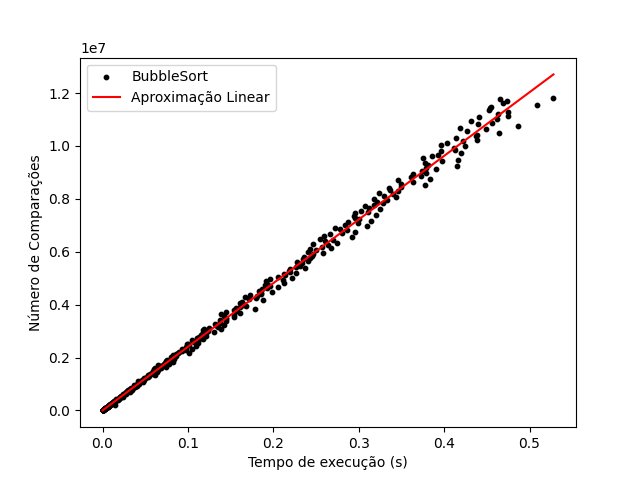
\includegraphics[width=0.7\textwidth]{FigTNB.png} 
\end{center}
\caption{Relação entre o número de comparações realizadas e o tempo de execução do \textit{BubbleSort}}
\label{fig:ntb}
\end{figure}

\begin{figure}[H]
\begin{center}
    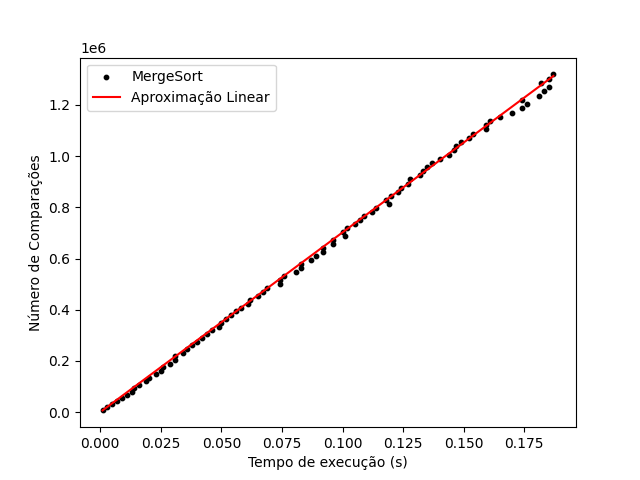
\includegraphics[width=0.7\textwidth]{FigTNM.png} 
\end{center}
\caption{Relação entre o número de comparações realizadas e o tempo de execução do \textit{MergeSort}}
\label{fig:ntm}
\end{figure}

\begin{figure}[H]
\begin{center}
    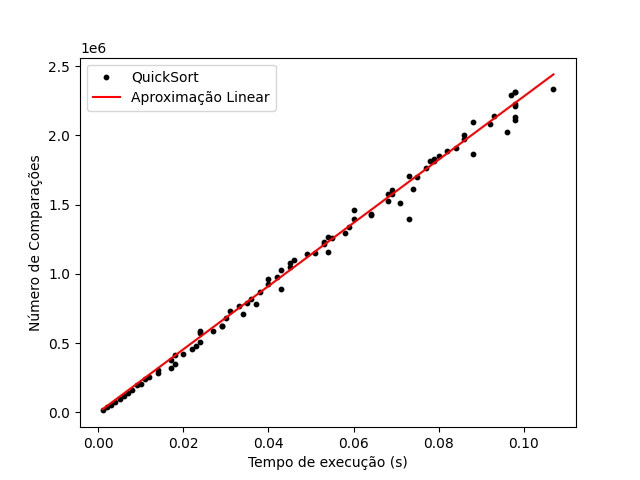
\includegraphics[width=0.7\textwidth]{FigTNQ.png} 
\end{center}
\caption{Relação entre o número de comparações realizadas e o tempo de execução do \textit{QuickSort}}
\label{fig:ntq}
\end{figure}

\subsection{BubbleSort}

\begin{table}[H]
\caption{Tamanho de \textit{array} de \textit{string} de entrada, o tempo para a execução do \textit{BubbleSort} em segundos e o número de comparações necessárias para ordenar o vetor }
\label{tab:db}
\begin{center}
\begin{tabular}{|c c c|}
\hline
Tamanho de \textit{array}	& Tempo (s)	& Comparações 	\\
\hline
1000 & 0.041 & 998001\\
2000 & 0.181 & 3996001\\
3000 & 0.393 & 8994001\\
4000 & 0.702 & 15992001\\
5000 & 1.100 & 24990001\\
6000 & 1.592 & 35988001\\
7000 & 2.149 & 48986001\\
8000 & 2.854 & 63984001\\
9000 & 3.542 & 80982001\\
10000 & 4.487 & 99980001\\
\hline
\end{tabular}
\end{center}
\end{table}

\quad A Tabela \ref{tab:db} demonstra o tempo de execução do \textit{BubbleSort} com \textit{array} de \textit{string} múltiplos de 1000, o gráfico da Figura \ref{fig:tb} mostra a relação entre o tempo para executar o algorítimo e o tamanho da entrada enquanto o gráfico da Figura \ref{fig:nb} mostra a relação entre o número de comparações realizadas e o tamanho da entrada.

\begin{figure}[H]
\begin{center}
    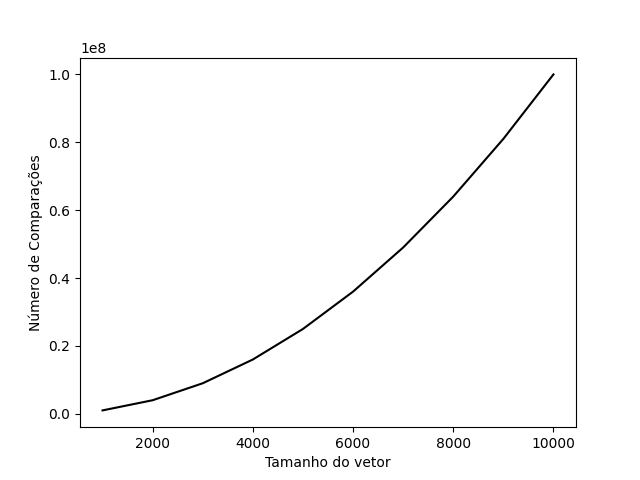
\includegraphics[width=0.7\textwidth]{FigNB.png} 
\end{center}
\caption{Relação entre o número de comparações realizadas pelo \textit{BubbleSort} e o tamanho da entrada}
\label{fig:nb}
\end{figure}

\begin{figure}[H]
\begin{center}
    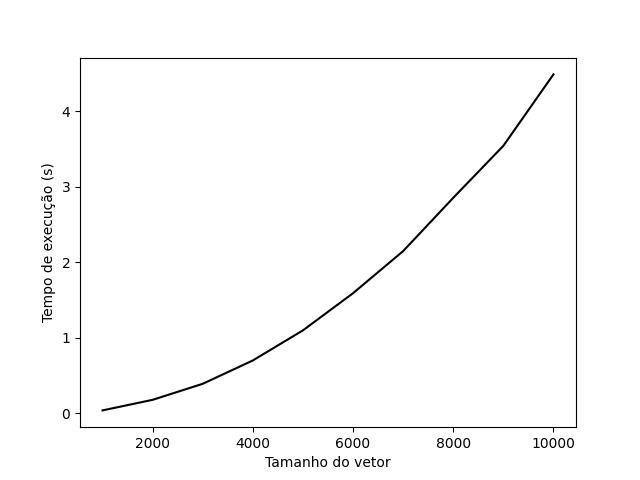
\includegraphics[width=0.7\textwidth]{FigTB.png} 
\end{center}
\caption{Relação entre o tempo de execução do \textit{BubbleSort} e o tamanho da entrada}
\label{fig:tb}
\end{figure}

\quad Ao sobrepor o gráfico encontrado na Figura \ref{fig:nb} com o gráfico de $f(x)=x^2$ obtêm-se a Figura \ref{fig:bOK}, percebe-se que ambas as curvas são semelhantes, isso se deve ao funcionamento do \textit{BubbleSort}, que garante que o número de comparações será sempre de $(n-1)^2$, onde $n$ é o tamanho do \textit{array} de entrada. De fato, os dados da Tabela \ref{tab:db} mostram essa exata relação.

\begin{figure}[H]
\begin{center}
    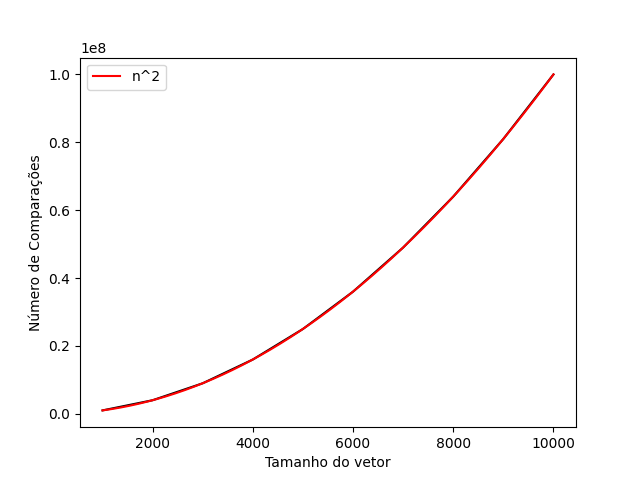
\includegraphics[width=0.7\textwidth]{FigBn2.png} 
\end{center}
\caption{Relação entre o número de comparações realizadas e o tamanho da entrada, com a função $f(x)=x^2$ evidenciada}
\label{fig:bOK}
\end{figure}

\subsection{MergeSort}

\begin{table}[H]
\caption{Tamanho de \textit{array} de \textit{string} de entrada, o tempo para a execução do \textit{MergeSort} em segundos e o número de comparações necessárias para ordenar o vetor}
\label{tab:dm}
\begin{center}
\begin{tabular}{|c c c|}
\hline
Tamanho de \textit{array}	& Tempo (s)	& Comparações 	\\
\hline
100000 & 0.217 & 1536691\\
200000 & 0.460 & 3272186\\
300000 & 0.709 & 5084573\\
400000 & 0.966 & 6945165\\
500000 & 1.387 & 8837351\\
600000 & 1.497 & 10769256\\
700000 & 1.827 & 12722702\\
800000 & 2.038 & 14690740\\
900000 & 2.460 & 16678844\\
1000000 & 2.574 & 18674058\\
\hline
\end{tabular}
\end{center}
\end{table}

\quad A Tabela \ref{tab:dm} demonstra o tempo de execução do \textit{MergeSort} com \textit{array} de \textit{string} múltiplos de 100000, o gráfico da Figura \ref{fig:tm} mostra a relação entre o tempo para executar o algorítimo e o tamanho da entrada enquanto o gráfico da Figura \ref{fig:nm} mostra a relação entre o número de comparações realizadas e o tamanho da entrada.

\begin{figure}[H]
\begin{center}
    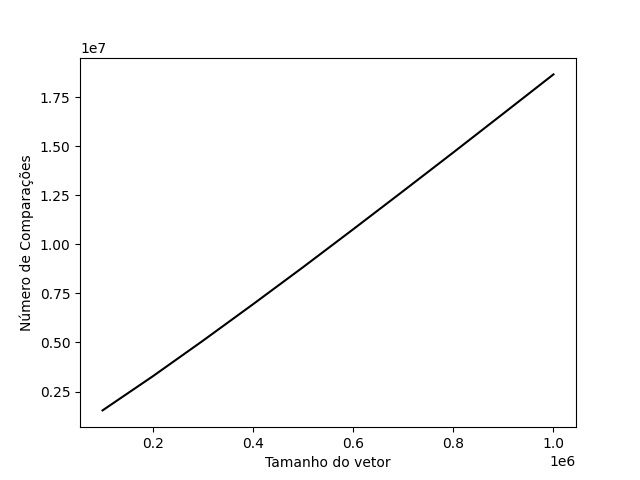
\includegraphics[width=0.7\textwidth]{FigNM.png} 
\end{center}
\caption{Relação entre o número de comparações realizadas pelo \textit{MergeSort} e o tamanho da entrada}
\label{fig:nm}
\end{figure}

\begin{figure}[H]
\begin{center}
    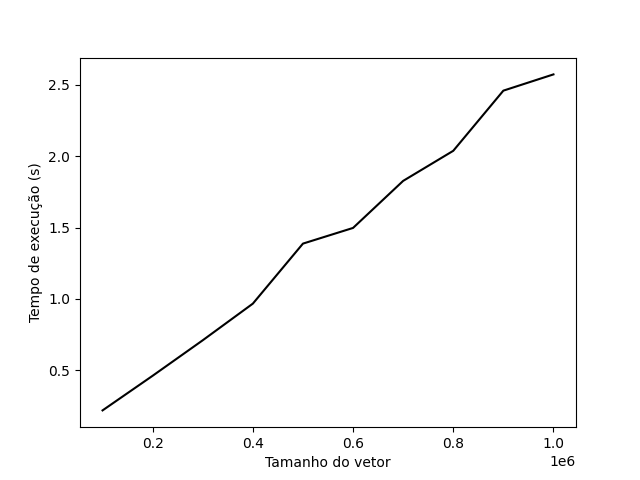
\includegraphics[width=0.7\textwidth]{FigTM.png} 
\end{center}
\caption{Relação entre o tempo de execução do \textit{MergeSort} e o tamanho da entrada}
\label{fig:tm}
\end{figure}

\quad Apesar de, no olhar, a relação exposta em \ref{fig:nm} parecer linear, quando se sobrepõe um gráfico semelhante com tamanhos de \textit{array} menores com o gráfico de $f(x)=x\log{(x)}$ obtêm-se a Figura \ref{fig:mOK}, que torna evidente a relação entre as duas curvas. De fato, ao se tabelar os dados da Tabela \ref{tab:dm} tratando-os conforme a função prevista, cria-se a Tabela \ref{tab:mOK}, mostrando ainda mais a equivalência.

\begin{figure}[H]
\begin{center}
    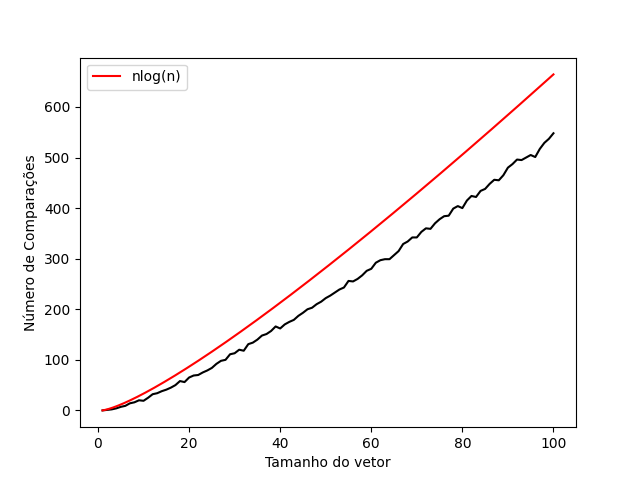
\includegraphics[width=0.7\textwidth]{FigMnlogn.png} 
\end{center}
\caption{Relação entre o número de comparações realizadas e o tamanho da entrada, com a função $f(x)=x\log{(x)}$ evidenciada}
\label{fig:mOK}
\end{figure}

\begin{table}[H]
\caption{Comparação entre o número esperado de comparações e o número real seguindo $O(n\log{(n)})$}
\label{tab:mOK}
\begin{center}
\begin{tabular}{|c c|}
\hline
$n\log{(n)}$ & Comparações \\
\hline
1660964 & 1536691\\
3521928 & 3272186\\
5458380 & 5084573\\
7443856 & 6945165\\
9465784 & 8837351\\
11516761 & 10769256\\
13591896 & 12722702\\
15687712 & 14690740\\
17801608 & 16678844\\
19931568 & 18674058\\
\hline
\end{tabular}
\end{center}
\end{table}

\subsection{QuickSort}

\begin{table}[H]
\caption{Tamanho de \textit{array} de \textit{string} de entrada, o tempo para a execução do \textit{QuickSort} em segundos e o número de comparações necessárias para ordenar o vetor }
\label{tab:dq}
\begin{center}
\begin{tabular}{|c c c|}
\hline
Tamanho de \textit{array}	& Tempo (s)	& Comparações 	\\
\hline
100000 & 0.118 & 2813431\\
200000 & 0.246 & 5987814\\
300000 & 0.394 & 9267216\\
400000 & 0.529 & 13331229\\
500000 & 0.713 & 16357150\\
600000 & 0.809 & 20266377\\
700000 & 0.996 & 24379843\\
800000 & 1.183 & 29151141\\
900000 & 1.309 & 33478205\\
1000000 & 1.450 & 36806554\\
\hline
\end{tabular}
\end{center}
\end{table}

\quad A Tabela \ref{tab:dq} demonstra o tempo de execução do \textit{QuickSort} com \textit{array} de \textit{string} múltiplos de 100000, o gráfico da Figura \ref{fig:tq} mostra a relação entre o tempo para executar o algorítimo e o tamanho da entrada enquanto o gráfico da Figura \ref{fig:nq} mostra a relação entre o número de comparações realizadas e o tamanho da entrada.

\begin{figure}[H]
\begin{center}
    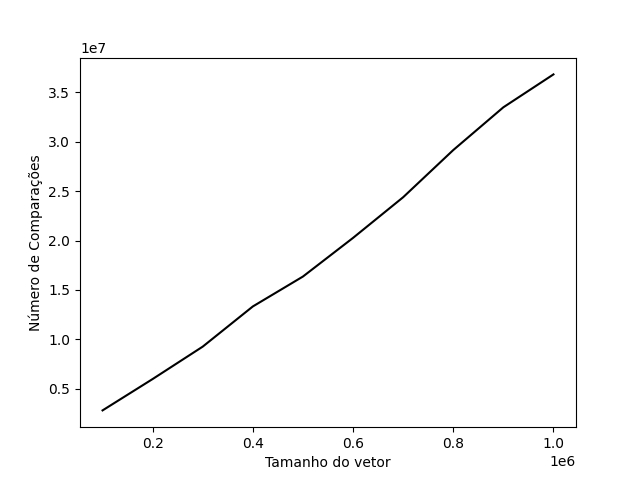
\includegraphics[width=0.7\textwidth]{FigNQ.png} 
\end{center}
\caption{Relação entre o número de comparações realizadas pelo \textit{QuickSort} e o tamanho da entrada}
\label{fig:nq}
\end{figure}

\begin{figure}[H]
\begin{center}
    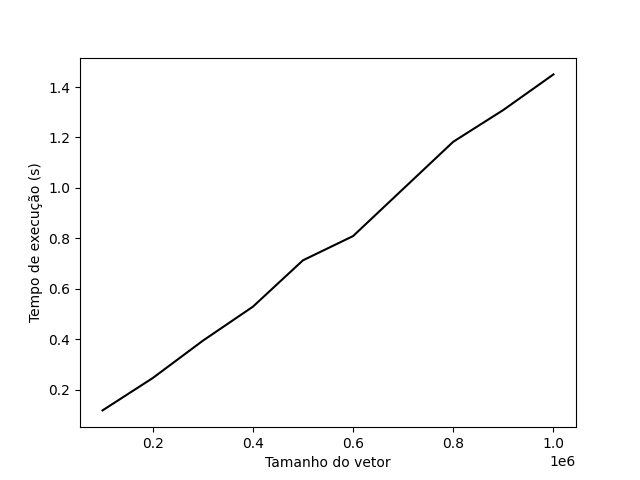
\includegraphics[width=0.7\textwidth]{FigTQ.png} 
\end{center}
\caption{Relação entre o tempo de execução do \textit{QuickSort} e o tamanho da entrada}
\label{fig:tq}
\end{figure}

\quad Apesar de, no olhar, a relação exposta em \ref{fig:nq} parecer linear, quando se sobrepõe um gráfico semelhante com tamanhos de \textit{array} menores com o gráfico de $f(x)=x\log{(x)}$ obtêm-se a Figura \ref{fig:qOK}, que torna mais claro a relação entre as duas curvas. A figura, ainda assim, possui um ruído muito grande quando comparado à função esperada, isso se deve ao fato de apenas o caso médio e melhor caso do \textit{QuickSort} ser $O(n\log{(n)})$, enquanto o pior caso possui complexidade de $O(n^2))$, correspondendo aos picos observados.

\begin{figure}[H]
\begin{center}
    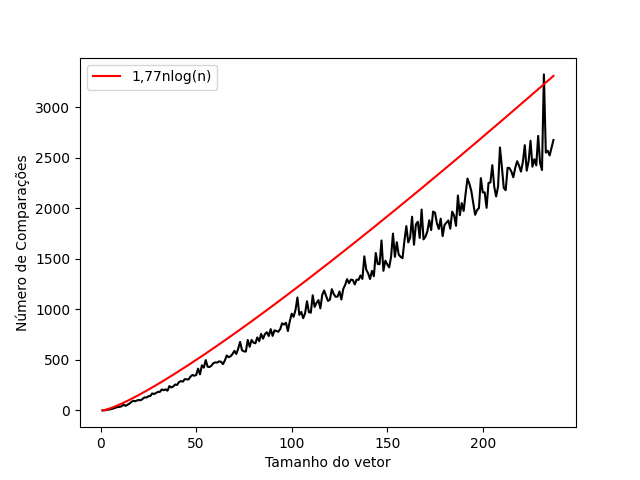
\includegraphics[width=0.7\textwidth]{FigQnlogn.png} 
\end{center}
\caption{Relação entre o número de comparações realizadas e o tamanho da entrada, com a função $f(x)=x\log{(x)}$ evidenciada}
\label{fig:qOK}
\end{figure}

\section{Conclusão}

\quad Após as analises feitas nesse relatório, pode-se concluir que a relação entre tempo e número de comparações é linear, porém, nem toda operação possui o mesmo tempo, uma vez que, o \textit{QuickSort}, apesar de possuir mais comparações do que o \textit{MergeSort}, possui tempo de execução menor, isso é decorrente do fato de que o \textit{MergeSort} copia as \textit{string} diversas vezes em \textit{array} auxiliar, sendo essa operação muito mais demorada.

\quad Portanto, para o fim que esse relatório se propôs a analisar, ordenação de \textit{array} de \textit{string}, o \textit{QuickSort} é, em média, o melhor dentre os métodos analisados.



\end{document}

